\documentclass[a4paper, 12pt]{report}

\usepackage{cmap}
\usepackage[russian]{babel}
\usepackage[T2A]{fontenc}
\usepackage[utf8]{inputenc}

\usepackage[left=2cm, right=1cm, top=2cm, bottom=1cm]{geometry}
\setlength{\footskip}{15pt}

\usepackage{setspace}
\onehalfspacing

\usepackage{pdflscape}

\usepackage[unicode]{hyperref}

\usepackage{xcolor}
\usepackage{pagecolor}

\usepackage{graphicx}

\usepackage{listings}

\hypersetup{
	pdftitle={Бинарные числа и их применение},
	pdfauthor={Какнаев Артем Владимирович},
	pdfkeywords={бинарная система, информатика, числа},
	colorlinks=true,
	linkcolor=blue,
	urlcolor=blue
}

\usepackage{multirow}

\begin{document}
	
	\begin{titlepage}
		
		\begin{center}
			
			{\large
				Петрозаводский Государственный университет
				
				Институт математики и информационных технологий
			}\\
			
			Направление подготовки бакалавриата \\
			09.03.04 - Программная инженерия \\
			
			\vfill
			
			{\large
				Практическая работа
				
				Бинарные числа и их применение
			}
			
			\vfill
			
			\begin{flushright}
				\parbox{9 cm}{
				Выполнил:\\
				студент 1 курса группы 22107 \\
				Какнаев Артем Владимирович
				
				\vspace{1cm}
				
				Проверил: \\
				Преподаватель Чистяков Дмитрий Борисович
			}
			\end{flushright}

			\vfill
			{\large
				Петрозаводск - 2026
			}
			
		\end{center}
		
	\end{titlepage}
	
	\tableofcontents
	\newpage
	
	
	\chapter{Введение}	
	Бинарная система счисления играет ключевую роль в современной информатике и вычислительной технике. 
	Все цифровые устройства, \textcolor{red}{включая компьютеры, смартфоны и микроконтроллеры,} используют именно эту систему 
	для хранения и обработки информации.
	
	В отличие от десятичной системы, привычной для человека, бинарная система оперирует всего двумя символами: 
	нулём и единицей. Это значительно упрощает реализацию вычислений на уровне электронных схем, так как 
	физически удобно представлять два состояния: есть сигнал или нет сигнала.
	
	Актуальность изучения бинарной системы обусловлена тем, что она лежит в основе всех современных технологий. 
	Понимание принципов её работы позволяет лучше разобраться в том, как функционируют компьютеры, как 
	происходит обработка данных и каким образом реализуются арифметические операции.
	
	\colorbox{yellow}{Целью работы является изучение бинарной системы счисления и её применения.}
	
	\chapter{Основная часть}
	\textcolor{red}{Бинарная система счисления — это позиционная система, в которой используются только две цифры: 0 и 1.}
	Каждая позиция числа имеет вес, равный степени числа 2, начиная с нулевой степени справа налево.
	
	Например, число 101 в двоичной системе можно представить как сумму степеней двойки:
	первая единица соответствует $2^2$, ноль — $2^1$, последняя единица — $2^0$ (некоторые переводы чисел представлены в таблице \ref{tab:one}).
	Таким образом, это число равно 5 в десятичной системе. Алгоритм, реализованный на языке C для перевода числа в двоичную систему, представлен в \ref{lst:bin} 
	
	Бинарные числа широко используются в вычислительной технике, поскольку электронные компоненты 
	легко реализуют два устойчивых состояния. Это позволяет надёжно хранить и передавать информацию.
	
	Кроме того, бинарная система лежит в основе представления различных типов данных: целых чисел, 
	вещественных чисел, текстовой информации и даже изображений. Любые данные в компьютере в конечном 
	итоге преобразуются в последовательности нулей и единиц.
	
	Преобразование чисел из десятичной системы в двоичную осуществляется путём последовательного деления 
	на 2 с записью остатков. Обратное преобразование выполняется через суммирование степеней двойки.
	
	Таким образом, бинарная система является фундаментом всей цифровой техники и играет важную роль 
	в области программирования и компьютерных наук.
	
	С дополнительной информацией можно ознакомиться на сайте:
	\url{https://otus.ru/journal/dvoichnaya-sistema-schisleniya-i-binarnyj-kod-chto-nuzhno-znat-novichku/}
	
	\section{Преимущества и особенности бинарной системы}
	
	\begin{enumerate}
		\item Простота реализации
		\begin{enumerate}
			\item Используется только два состояния
			\item Легко реализуется на электронных схемах
		\end{enumerate}
		
		\item Надёжность хранения данных
		\begin{enumerate}
			\item Устойчивость к помехам
			\item Простота проверки ошибок
		\end{enumerate}
		
	\end{enumerate}
	
	\chapter{Применение бинарной системы}
	Бинарная система широко применяется в различных областях науки и техники. 
	В первую очередь она используется в компьютерах и цифровых устройствах.
	
	Все операции, выполняемые процессором, основаны на обработке бинарных данных. 
	Арифметические действия, логические операции и управление программами реализуются 
	с использованием двоичных чисел.
	
	Также бинарная система применяется в системах передачи данных. Информация передаётся 
	в виде электрических или оптических сигналов, которые интерпретируются как нули и единицы.
	
	\textcolor{red}{В области хранения информации бинарный код используется в жёстких дисках, SSD-накопителях 
	и оперативной памяти. Данные записываются в виде последовательностей битов, что обеспечивает 
	высокую скорость и надёжность хранения.}
	
	Таким образом, бинарная система является универсальным инструментом представления информации 
	в цифровом мире.
	
	\section{Области применения бинарных системы}
	\begin{itemize}
		\item Вычислительная техника
		\begin{itemize}
			\item Процессоры
			\item Оперативная память
		\end{itemize}
		
		\item Передача данных
		\begin{itemize}
			\item Сети передачи информации
			\item Интернет
		\end{itemize}
		
		\item Хранение информации
	\end{itemize}
	
	На рисунке \ref{fig:cpu} показаны процессор и оперативная память.
	
	\begin{figure}[h]
	\centering
	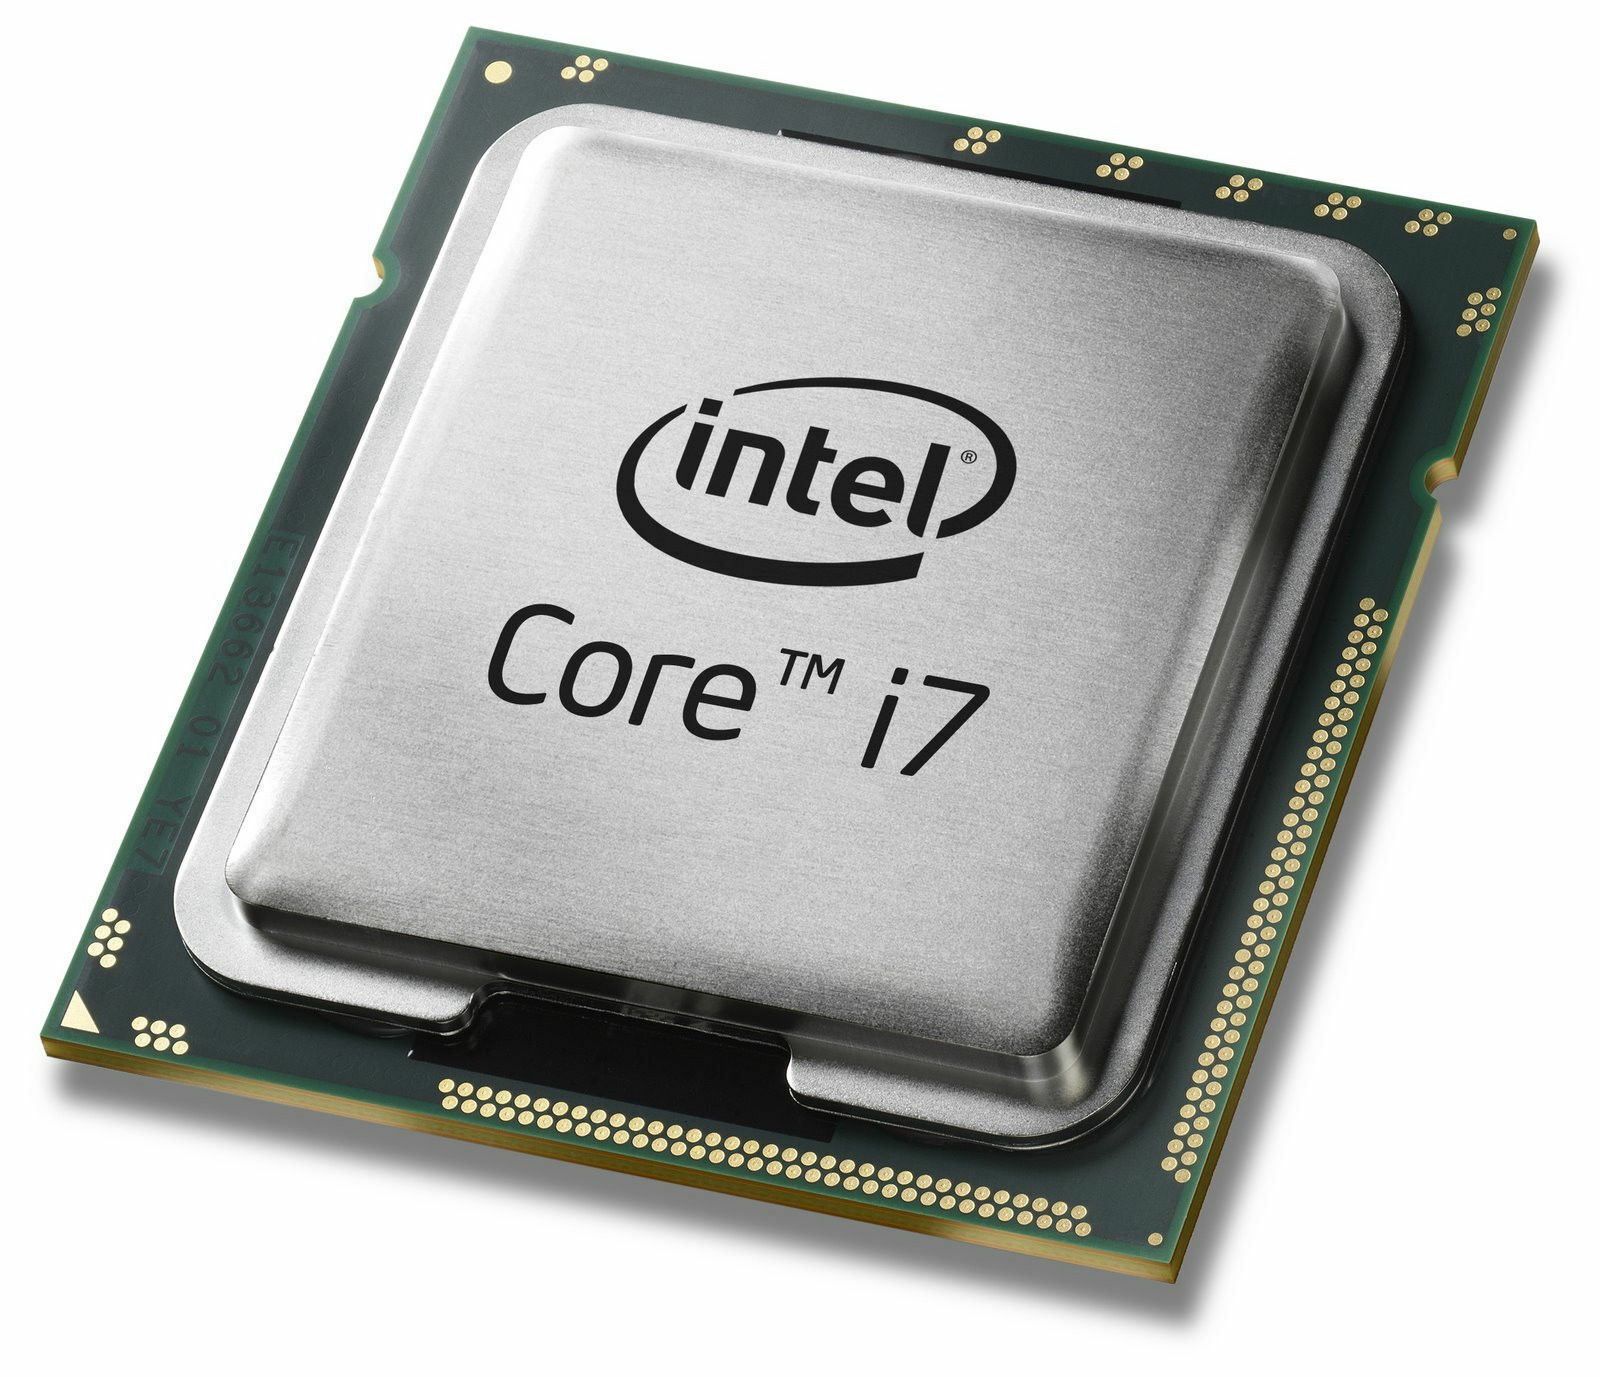
\includegraphics[width=0.5\textwidth]{image.png}
	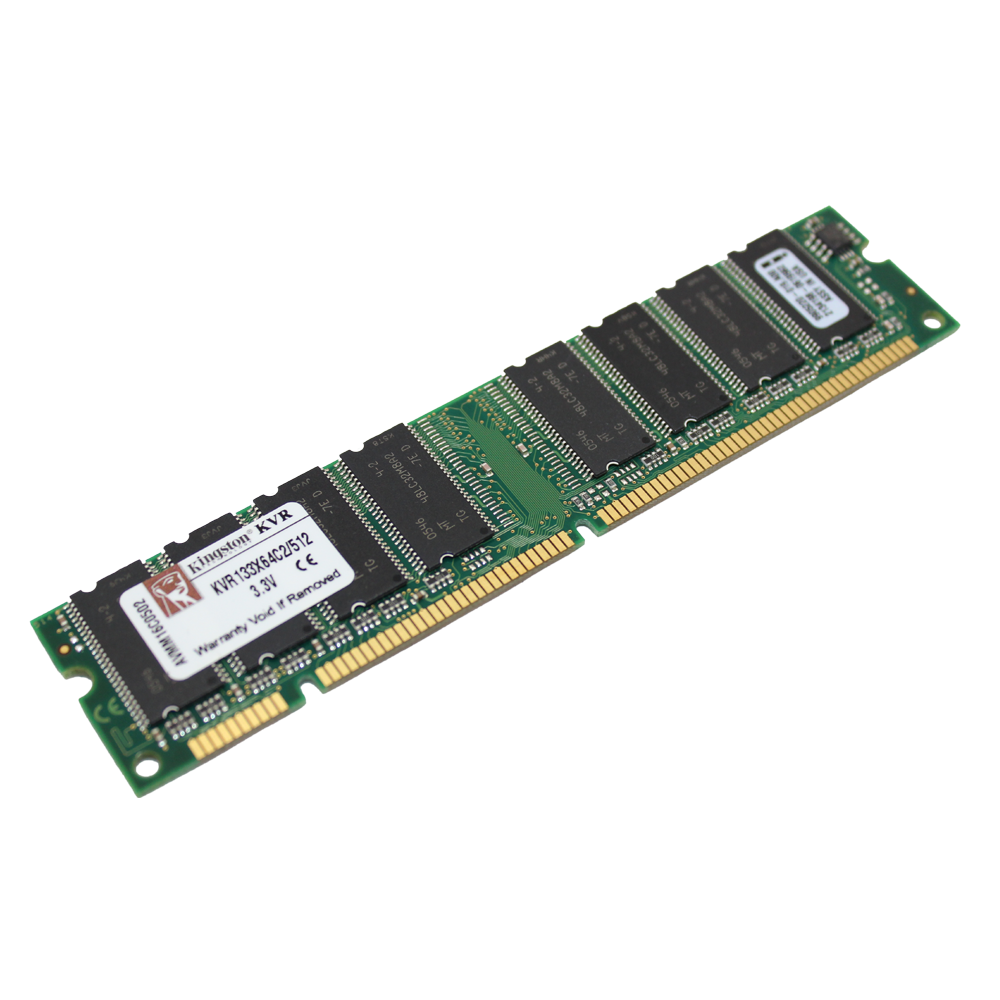
\includegraphics[width=0.5\textwidth]{image1.png}
	\caption{Процессор и оперативная память} 
	\label{fig:cpu}
	\end{figure}
	
	\begin{landscape}
		
		\pagestyle{plain}
	
		\chapter{Пример альбомной страницы}
		Альбомная ориентация страницы используется в тех случаях, когда необходимо разместить 
		широкие таблицы, схемы или графики.
		
		В рамках данной работы эта страница демонстрирует возможность изменения ориентации 
		документа. В дальнейшем здесь можно разместить таблицу с результатами вычислений 
		или сравнительный анализ различных систем счисления.
		
		Использование альбомной страницы позволяет более эффективно организовать пространство 
		документа при работе с широкими данными.
	\end{landscape}
	
	\chapter{Таблицы}
	
	\section{Простая таблица}
	
	\begin{table}[h]
		\centering
		\begin{tabular}{|c|c|c|}
		\hline
		Число (2) & Степень & Значение \\ \hline
		1 & $2^0$ & 1 \\ \hline
		10 & $2^1$ & 2 \\ \hline
		\multicolumn{2}{|c|}{Объединённая ячейка} & 4 \\ \hline
		\end{tabular}
		\caption{Пример таблицы с объединением столбцов}
		\label{tab:one}
	\end{table}
	
	\section{Объединение строк}
	
	\begin{table}[h]
		\centering
		\begin{tabular}{|c|c|}
			\hline
			\multirow{2}{*}{Бинарное число} & Значение \\ \cline{2-2}
											& 5 \\ \hline
			10 & 2 \\ \hline
		\end{tabular}
		\caption{Пример объединения строк}
		\label{tab:two}
	\end{table}
	
	\chapter{Математические основы бинарной системы}
	
	Бинарная система счисления тесно связана с математикой, в частности с теорией чисел и алгеброй.
	
	Любое натуральное число можно представить в виде суммы степеней двойки:
	
	\[
	N = a_n \cdot 2^n + a_{n-1} \cdot 2^{n-1} + \dots + a_0 \cdot 2^0
	\]
	
	где коэффициенты $a_i$ принимают значения 0 или 1.
	
	\section{Пример разложения}
	
	Рассмотрим число 13:
	
	\[
	13 = 1 \cdot 2^3 + 1 \cdot 2^2 + 0 \cdot 2^1 + 1 \cdot 2^0
	\]
	
	Следовательно, в двоичной системе:
	
	\[
	13_{10} = 1101_2
	\]
	
	\section{Арифметические операции}
	
	Сложение бинарных чисел выполняется по следующим правилам:
	
	\[
	0_2 + 0_2 = 0_2,\quad 1_2 + 0_2 = 1_2,\quad 1_2 + 1_2 = 10_2
	\]
	
	\section{Теорема}
	
	Любое натуральное число имеет единственное представление в двоичной системе счисления.
	
	Это утверждение следует из общей теоремы о представлении чисел в позиционных системах.
	
	\chapter{Пример программного кода}
	
	\section{Вывод на экран Hello, World!}
	\begin{lstlisting}
		#include <stdio.h>
		
		int main() {
			printf("Hello, World!");
			return 0;
		}
	\end{lstlisting}
	
	\section{Перевод числа в двоичную систему}
	\label{lst:bin}
	
	\begin{lstlisting}
		
		#include <stdio.h>
		int main() {
			int n, binary[32], i = 0;
			printf("Enter a number: ");
			scanf("%d", &n);
			while (n > 0) {
				binary[i] = n % 2;
				n = n / 2;
				i++;
			}
			printf("Binary: ");
			for (int j = i - 1; j >= 0; j--) {
				printf("%d", binary[j]);
			}
			return 0;
		}
	\end{lstlisting}
	
	\chapter{Визуализация графиков}
	
	\section{Функция одной переменной}
	
	График функции $y = x^2$
	
	\begin{figure}[h]
		\centering
		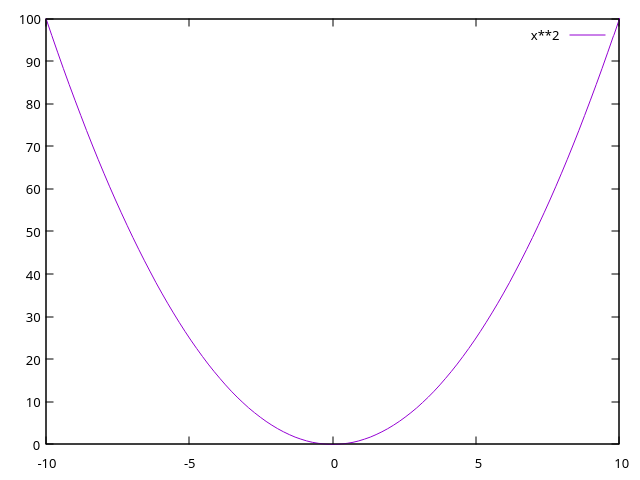
\includegraphics[width=0.6\textwidth]{parabola.png}
		\caption{График функции $y=x^2$}
		\label{fig:parabola}
	\end{figure}
	
	\newpage
	
	\section{Окружность}
	
	Параметрическое уравнение окружности:
	
	\begin{figure}[h]
		\centering
		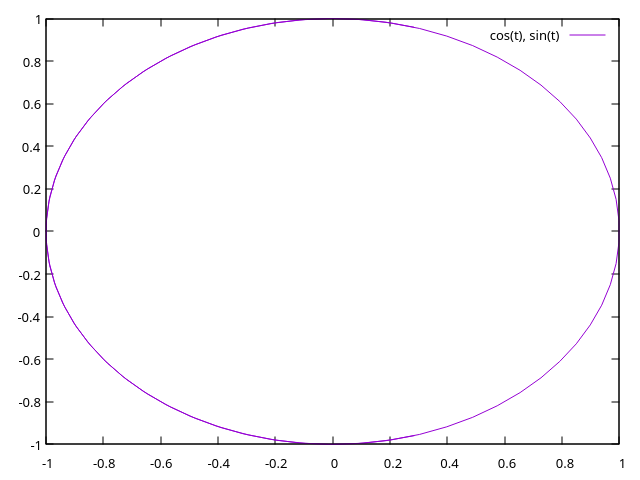
\includegraphics[width=0.6\textwidth]{circle.png}
		\caption{Параметрическая кривая (окружность)}
		\label{fig:circle}
	\end{figure}
	\newpage
	
	\section{Полярная координата}
	
	Пример спирали в полярной системе:
	\begin{figure}[h]
		\centering
		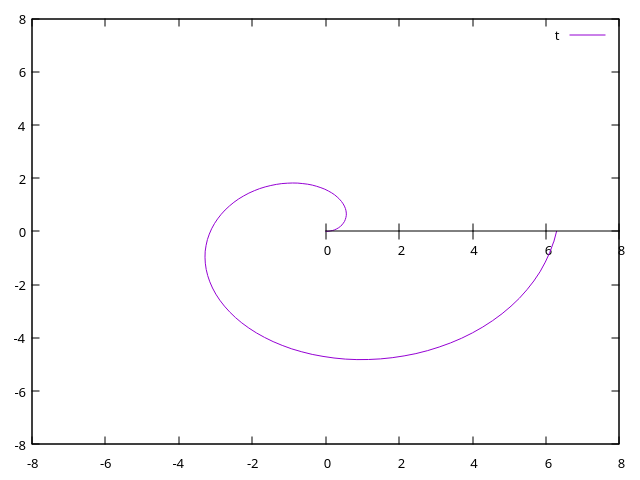
\includegraphics[width=0.6\textwidth]{spiral.png}
		\caption{Кривая в полярных координатах}
		\label{fig:spiral}
	\end{figure}
	
	\section{Поверхности}
	
	Пример поверхности $z = x^2 + y^2$:
	
	\begin{figure}[h]
		\centering
		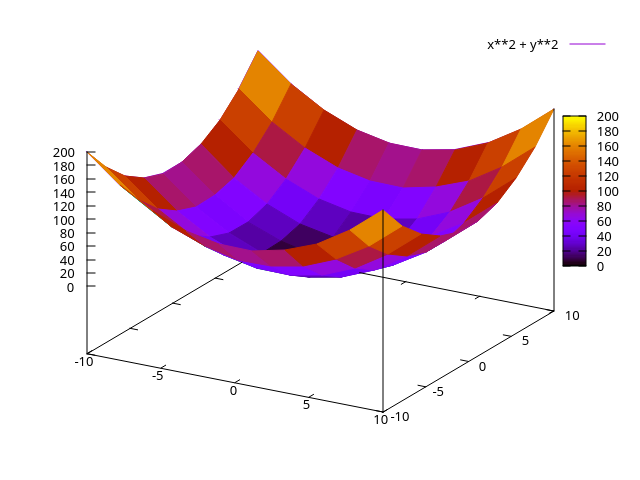
\includegraphics[width=0.6\textwidth]{surface.png}
		\caption{Поверхность}
	\end{figure}
	
	\newpage
	
	\section{Цилиндрические и сферические координаты}
	
	Цилиндр:
	
	\begin{figure}[h]
		\centering
		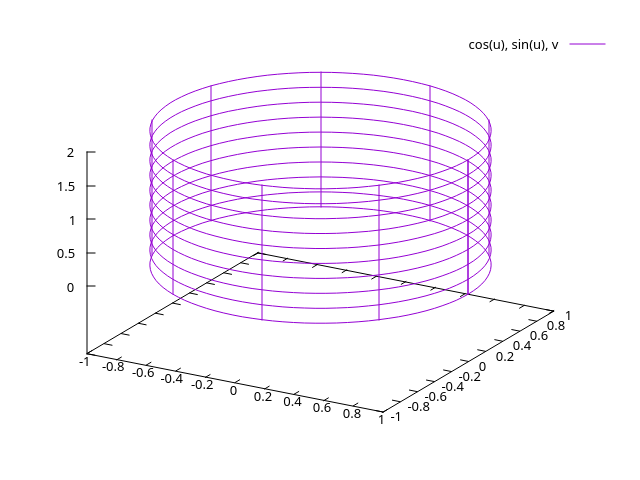
\includegraphics[width=0.6\textwidth]{cilinder.png}
		\caption{Цилиндр}
	\end{figure}
	
	Сфера:
	
	\begin{figure}[h]
		\centering
		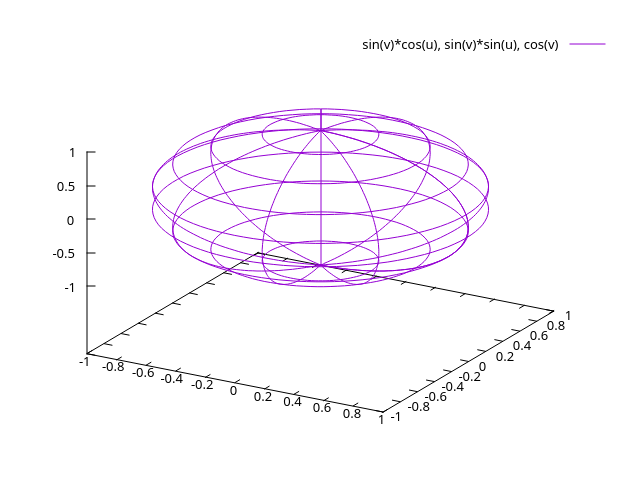
\includegraphics[width=0.7\textwidth]{sphere.png}
		\caption{Сфера}
	\end{figure}
	
	\chapter{Заключение}

	В ходе выполнения лабораторной работы была рассмотрена бинарная система счисления 
	и её роль в современной вычислительной технике.
	
	Было установлено, что использование всего двух состояний значительно упрощает 
	реализацию аппаратных и программных решений. Благодаря этому бинарная система 
	стала основой всех цифровых устройств.
	
	Также были рассмотрены основные принципы представления чисел и данных в двоичном виде, 
	а также области применения данной системы.
	
	Полученные знания являются фундаментальными для дальнейшего изучения информатики, 
	программирования и смежных дисциплин.
	
	\begin{thebibliography}{9}
	\pagecolor{yellow!30}
		
		\bibitem{knuth}
		Д. Кнут. Искусство программирования. Том 1. Основные алгоритмы.
		
		\bibitem{kolmogorov}
		А.Н. Колмогоров. Введение в теорию информации.
		
		\bibitem{site}
		\url{https://otus.ru/journal/dvoichnaya-sistema-schisleniya-i-binarnyj-kod-chto-nuzhno-znat-novichku/}
		
	\end{thebibliography}
	
\end{document}